%!TEX root = ../Thesis.tex
\section*{Anhang}
\addcontentsline{toc}{section}{Anhang}
\fancyhead[R]{Anhang}

\anhangsverzeichnis

\anhang{Weitere Use-Cases}\label{Anhang-Use-Cases}

\subanhang{Administrator}\label{Anhang-Admin}
\begin{figure}[h]
\centering
\begin{minipage}[t]{1\textwidth} 
\caption{Administrator - Use-Case Diagramm} 
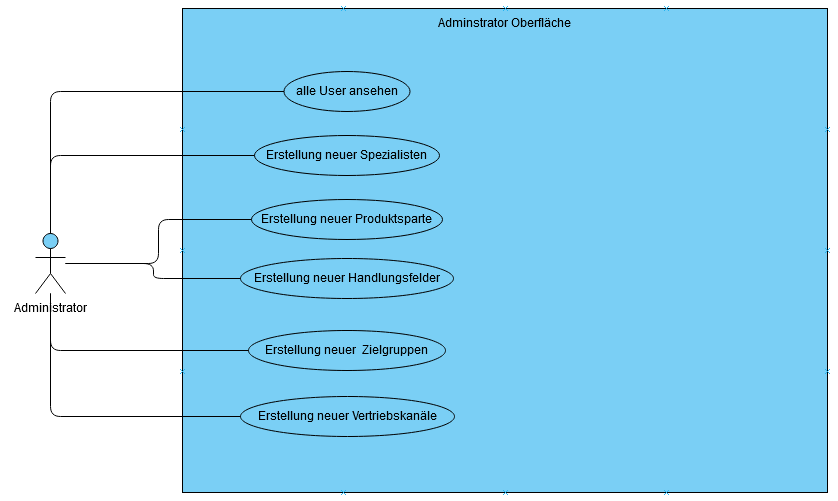
\includegraphics[width=1\textwidth]{img/admin-use-case.png}\\
\source{Eigene Darstellung} 
\end{minipage}
\end{figure}

\subanhang{Kontaktformular}\label{Anhang-Kontakt}
\begin{figure}[h]
\centering
\begin{minipage}[t]{1\textwidth} 
\caption{Kontaktformular - Use-Case Diagramm} 
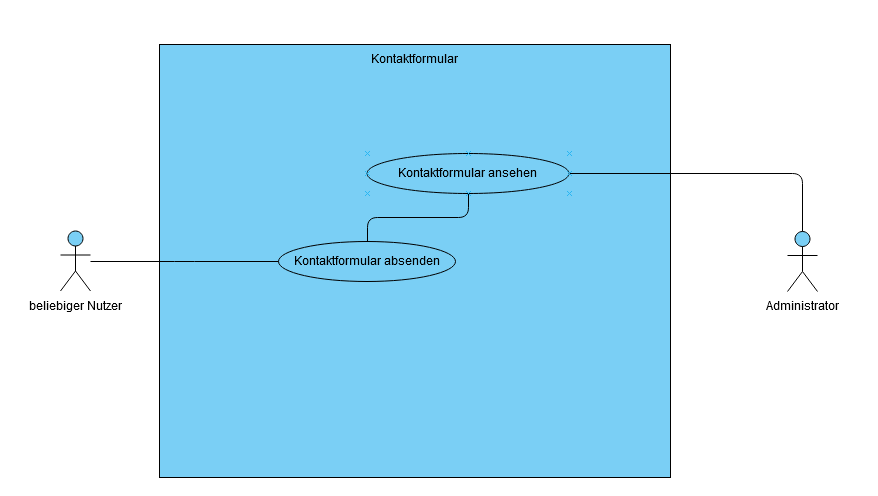
\includegraphics[width=1\textwidth]{img/kontakt-use-case.png}\\
\source{Eigene Darstellung} 
\end{minipage}
\end{figure}

\clearpage
\pagebreak

\anhang{GUI-Konzept}

\subanhang{Konzept}\label{GUI-Konzept}

\begin{figure}[hbt]
\centering
\begin{minipage}[t]{1\textwidth}
    \caption{GUI-Konzept - Login}
    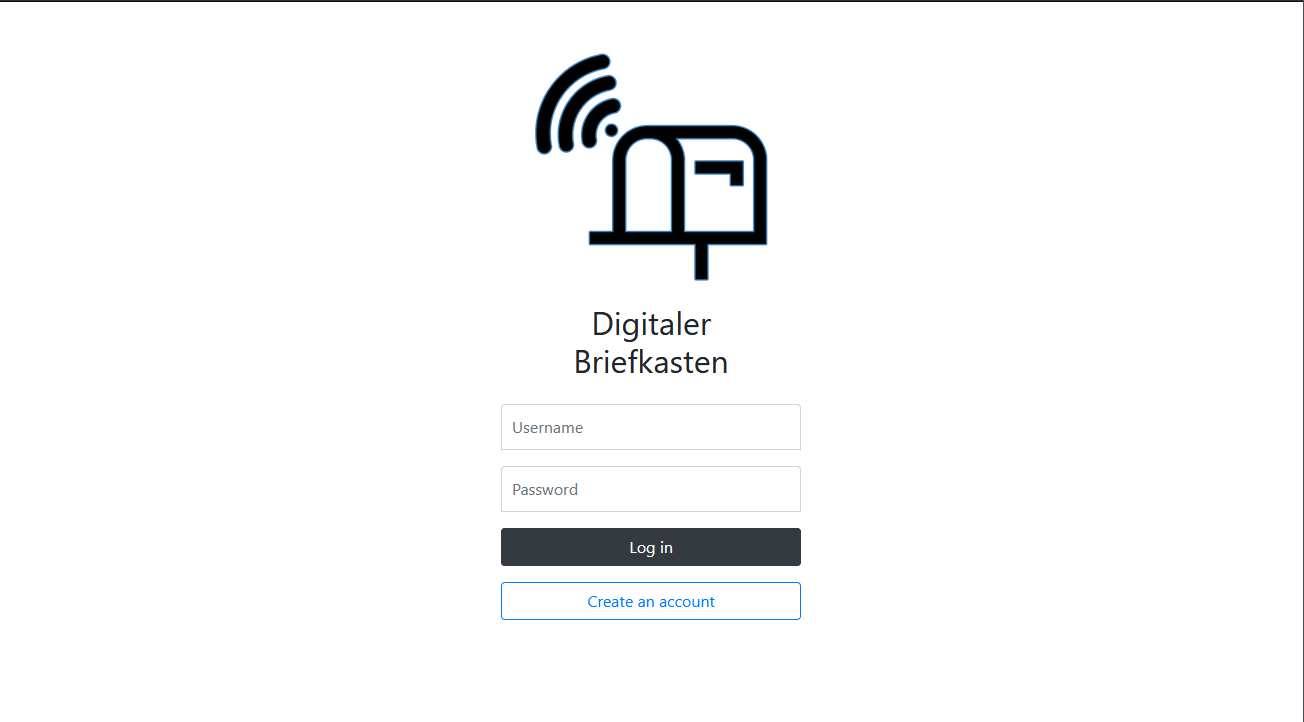
\includegraphics[width=1\textwidth]{img/login-konzept.png}\\
    \source{Eigene Darstellung}
    \label{fig:login}
\end{minipage}
\end{figure}

\begin{figure}[h]
\centering
\begin{minipage}[t]{1\textwidth} 
\caption{GUI-Konzept - Registrierung } 
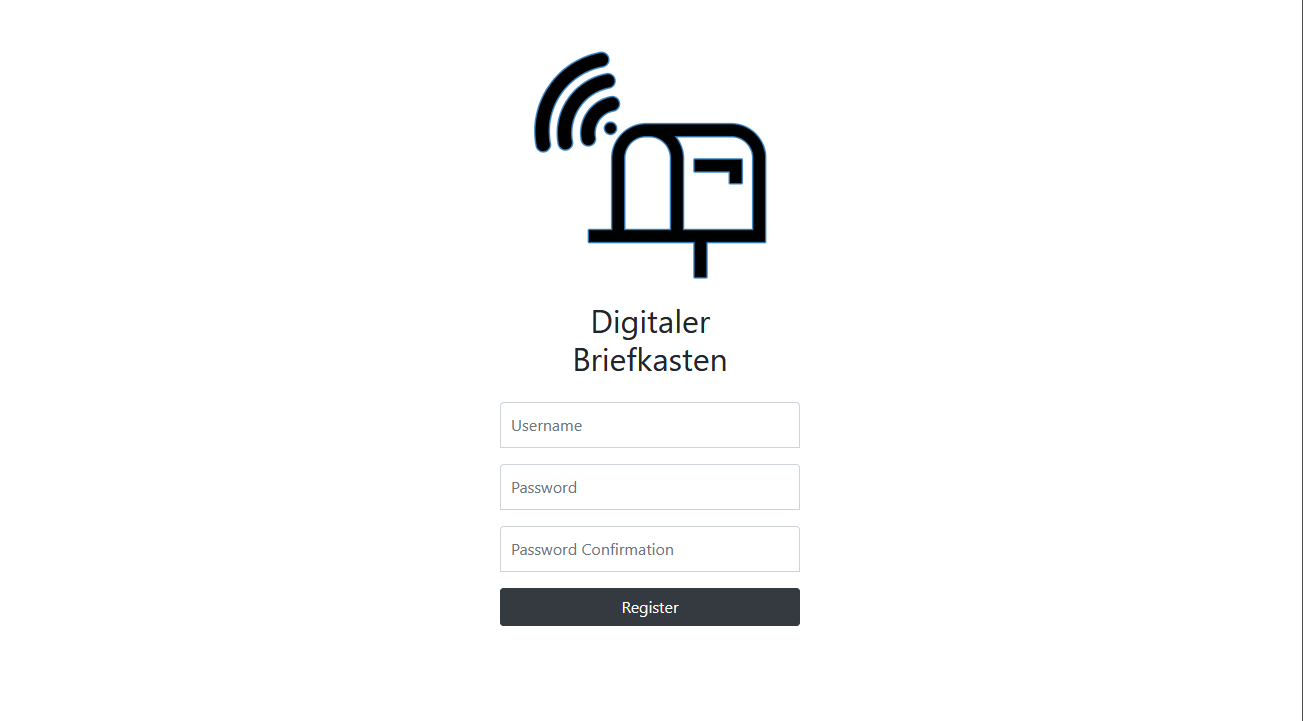
\includegraphics[width=1\textwidth]{img/registrierung-konzept.png}\\
\source{Eigene Darstellung} 
\end{minipage}
\end{figure}

\begin{figure}[h]
\centering
\begin{minipage}[t]{1\textwidth} 
\caption{GUI-Konzept - Willkommen} 
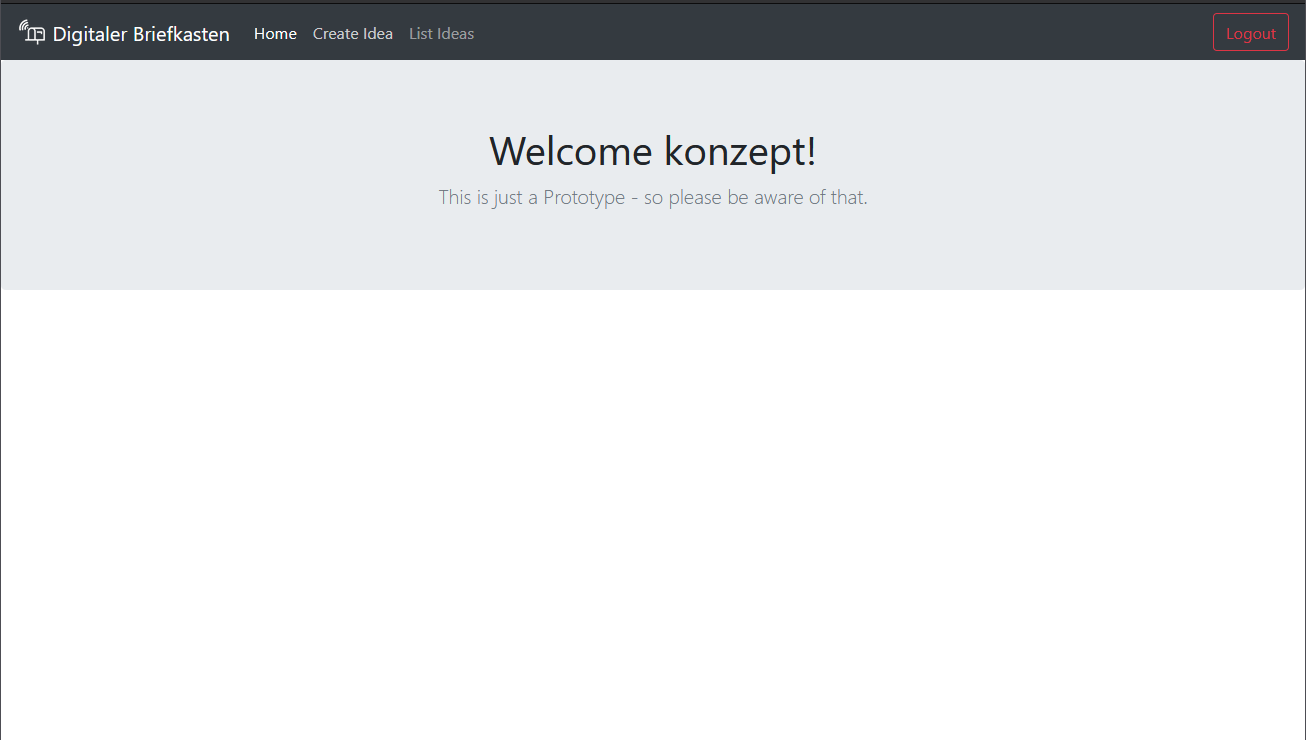
\includegraphics[width=1\textwidth]{img/welcome-konzept.png}\\
\source{Eigene Darstellung} 
\end{minipage}
\end{figure}

\begin{figure}[h]
\centering
\begin{minipage}[t]{1\textwidth} 
\caption{GUI-Konzept - Idee erstellen } 
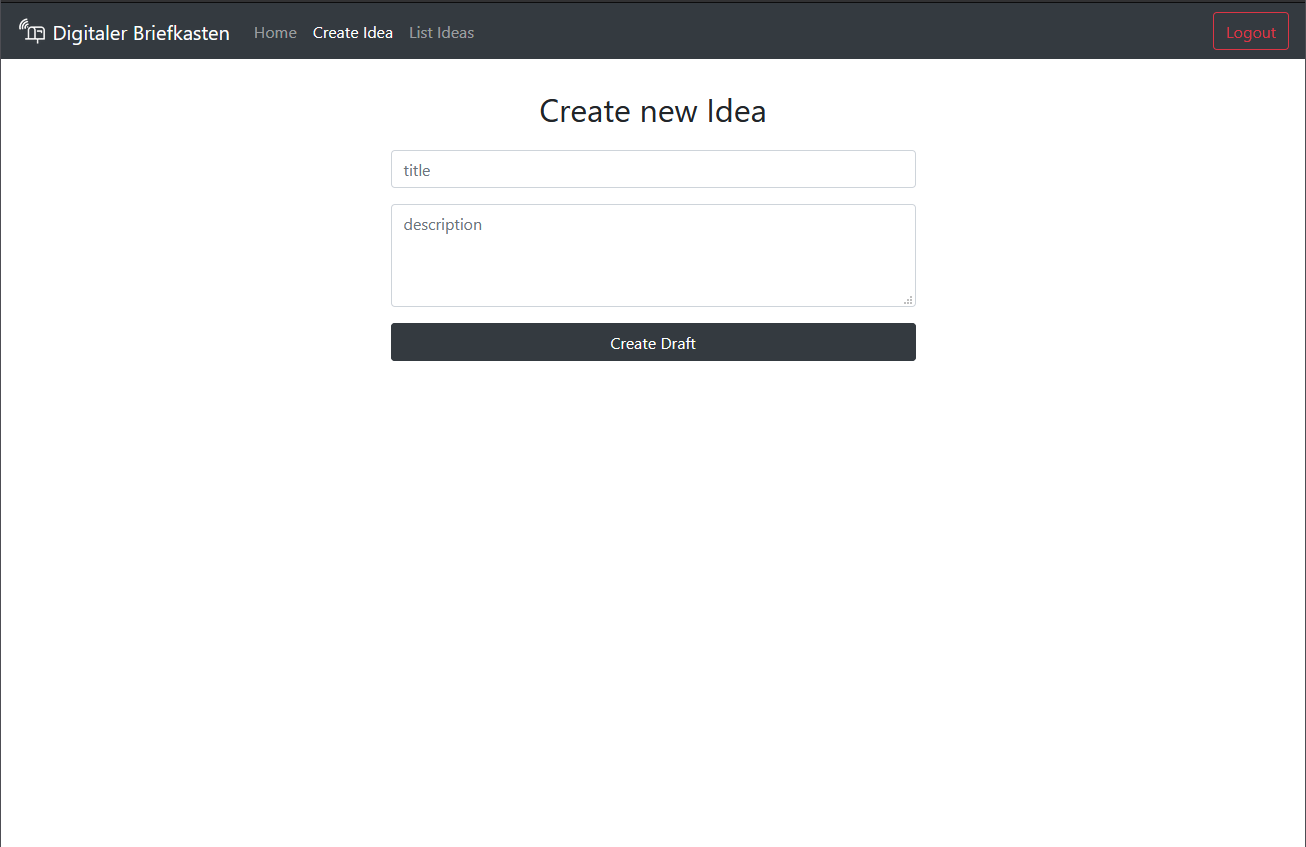
\includegraphics[width=1\textwidth]{img/createIdea-konzept.png}\\
\source{Eigene Darstellung} 
\end{minipage}
\end{figure}

\clearpage
\pagebreak

\subanhang{Umsetzung}\label{GUI-Umsetzung}

Die im folgenden dargestellten GUI Bestandteile stellen die wichtigsten Teile der Oberfläche dar. Auf die Abbildung aller Bestandteile wurde aufgrund der zu großen Menge, zur Wahrung der Übersichtlichkeit, verzichtet.

\begin{figure}[h]
\centering
\begin{minipage}[t]{1\textwidth} 
\caption{GUI-Umsetzung - Login } 
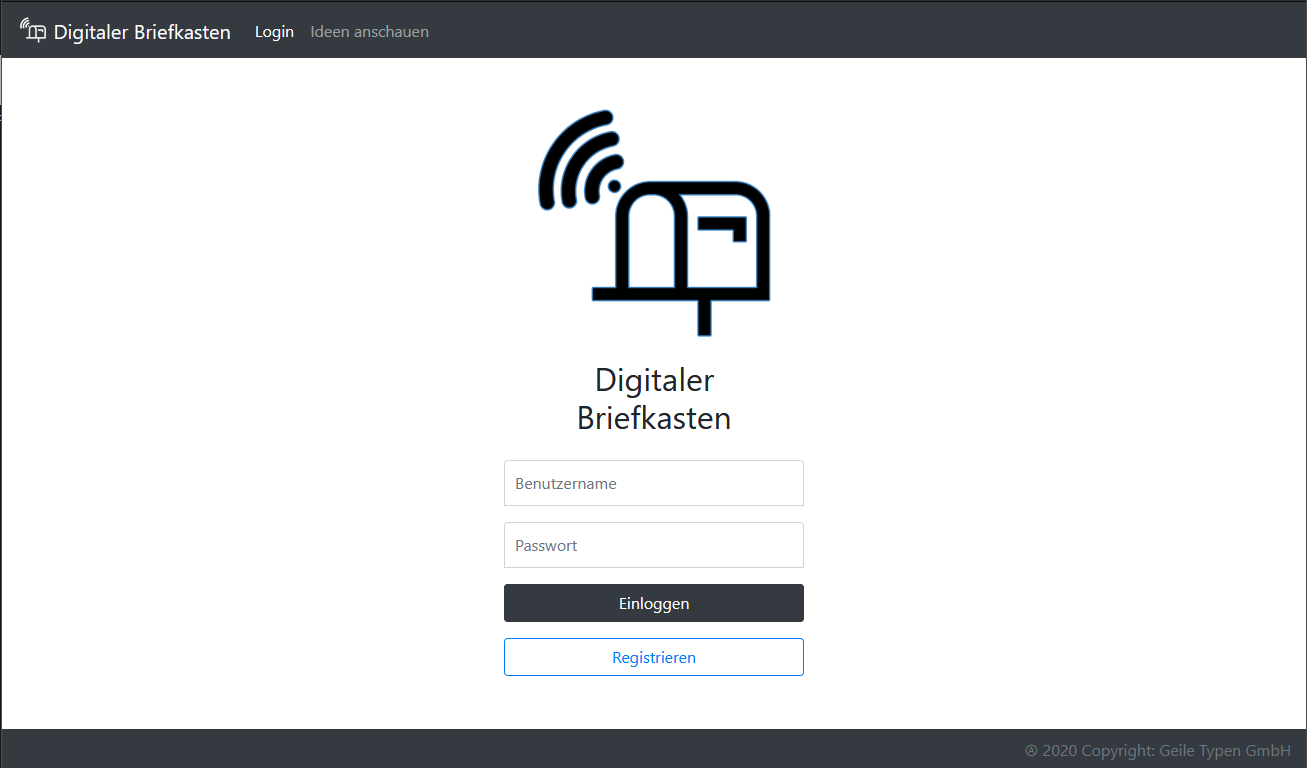
\includegraphics[width=1\textwidth]{img/login-umsetzung.png}\\
\source{Eigene Darstellung} 
\end{minipage}
\end{figure}

\begin{figure}[h]
\centering
\begin{minipage}[t]{1\textwidth} 
\caption{GUI-Umsetzung - Registrierung } 
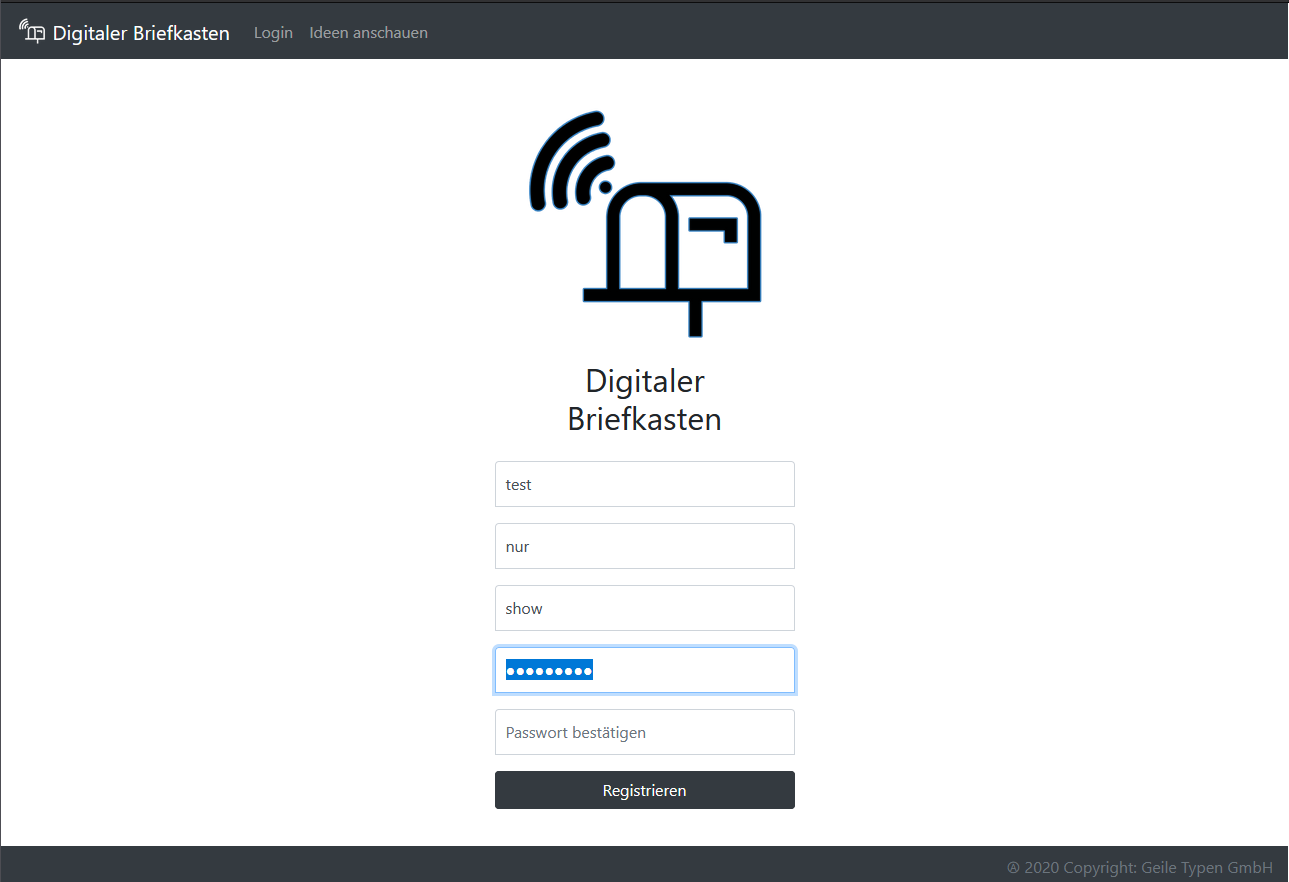
\includegraphics[width=1\textwidth]{img/registrierung-umsetzung.png}\\
\source{Eigene Darstellung} 
\end{minipage}
\end{figure}

\begin{figure}[h]
\centering
\begin{minipage}[t]{1\textwidth} 
\caption{GUI-Umsetzung - Ideen}
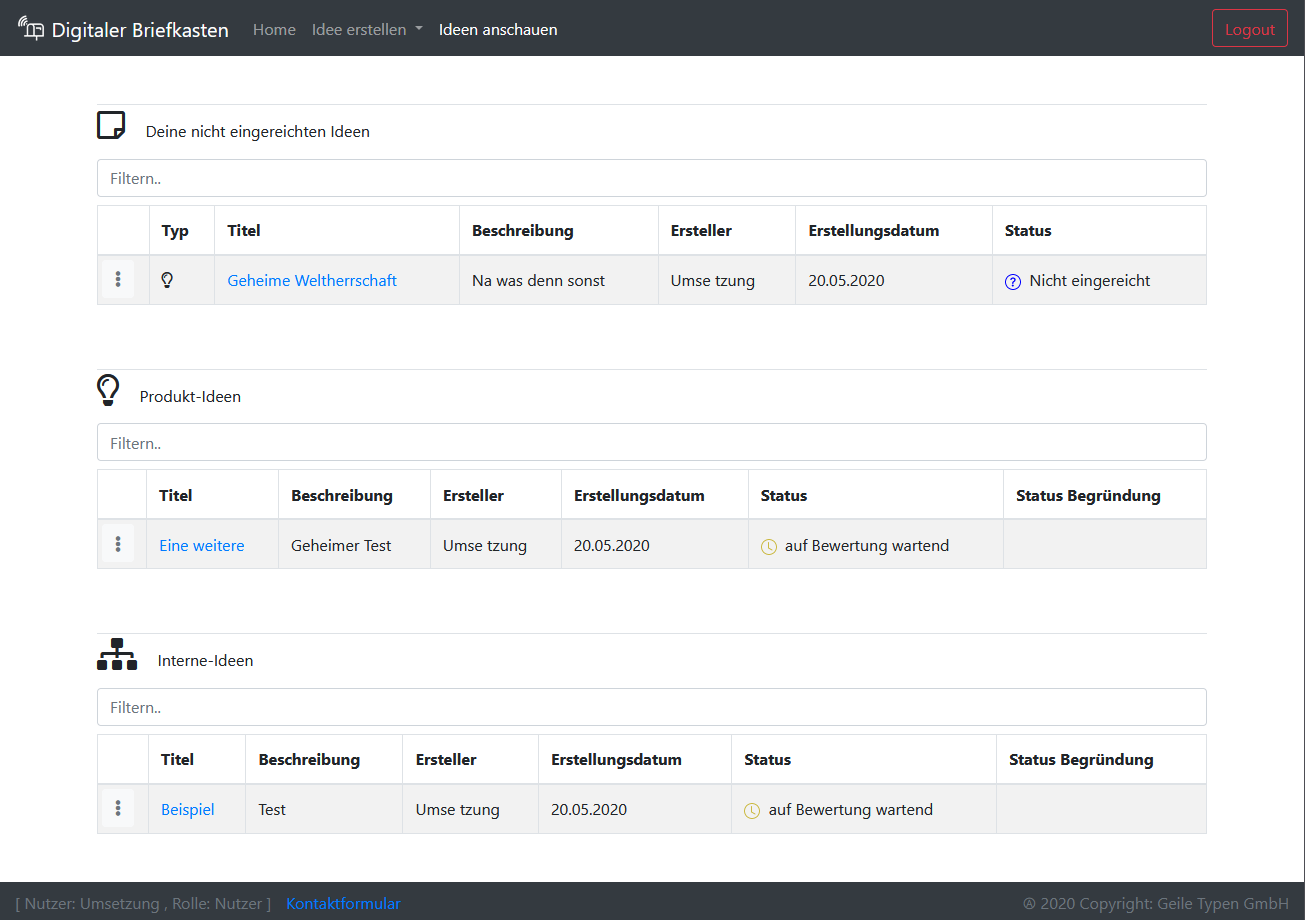
\includegraphics[width=1\textwidth]{img/ideen-umsetzung.png}\\
\source{Eigene Darstellung} 
\end{minipage}
\end{figure}

\begin{figure}[h]
\centering
\begin{minipage}[t]{1\textwidth} 
\caption{GUI-Umsetzung - Idee erstellen } 
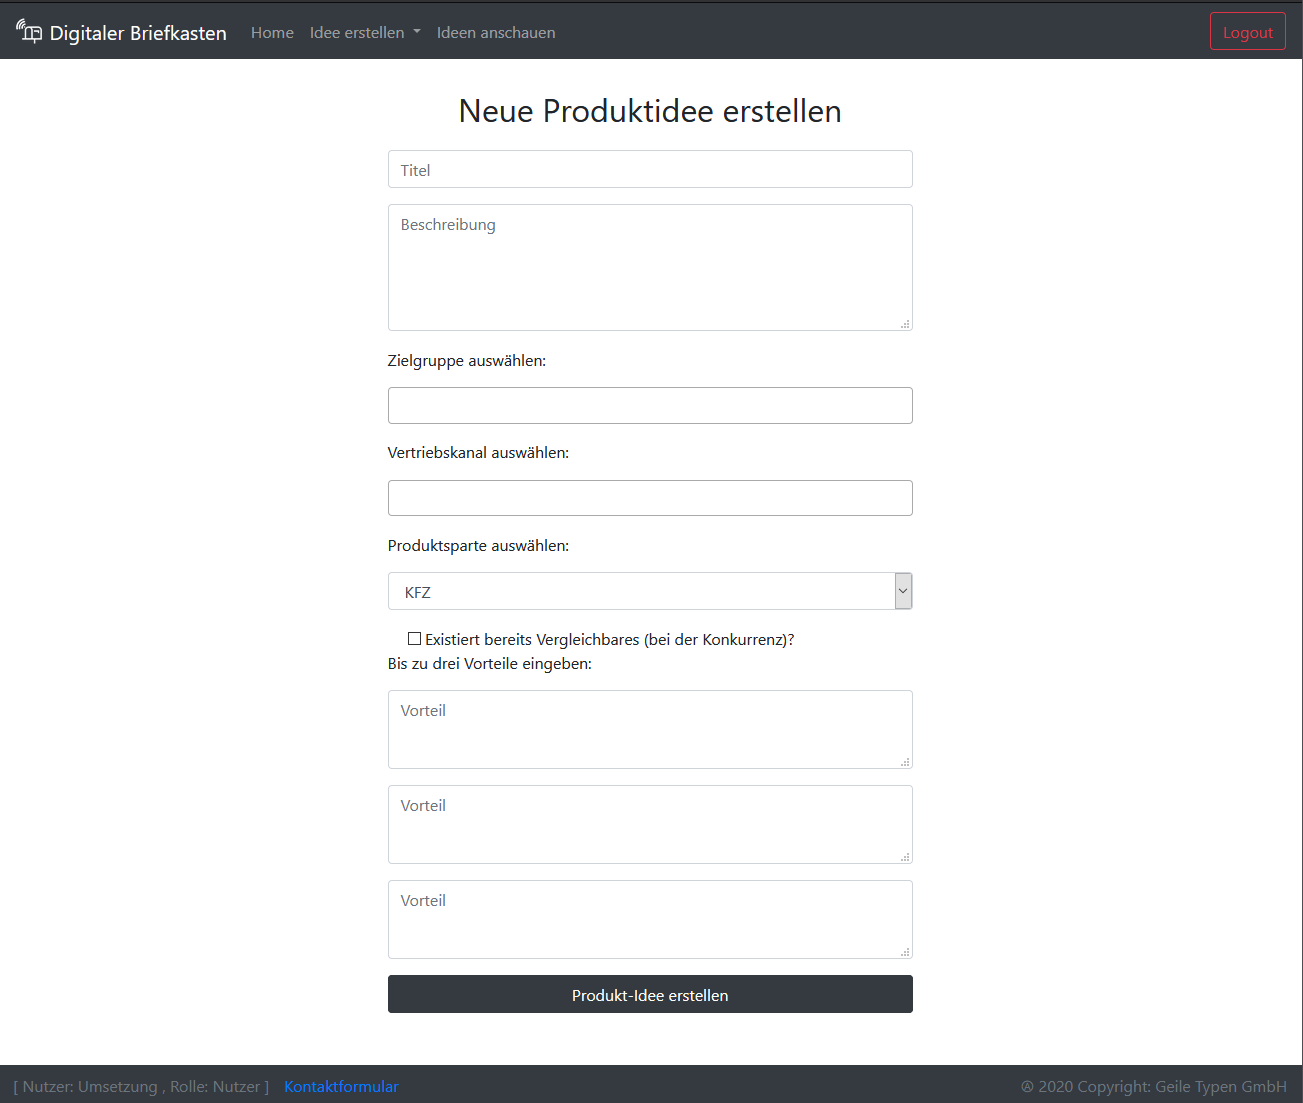
\includegraphics[width=1\textwidth]{img/createIdea-umsetzung.png}\\
\source{Eigene Darstellung} 
\end{minipage}
\end{figure}

\begin{figure}[h]
\centering
\begin{minipage}[t]{1\textwidth} 
\caption{GUI-Umsetzung - Idee ansehen } 
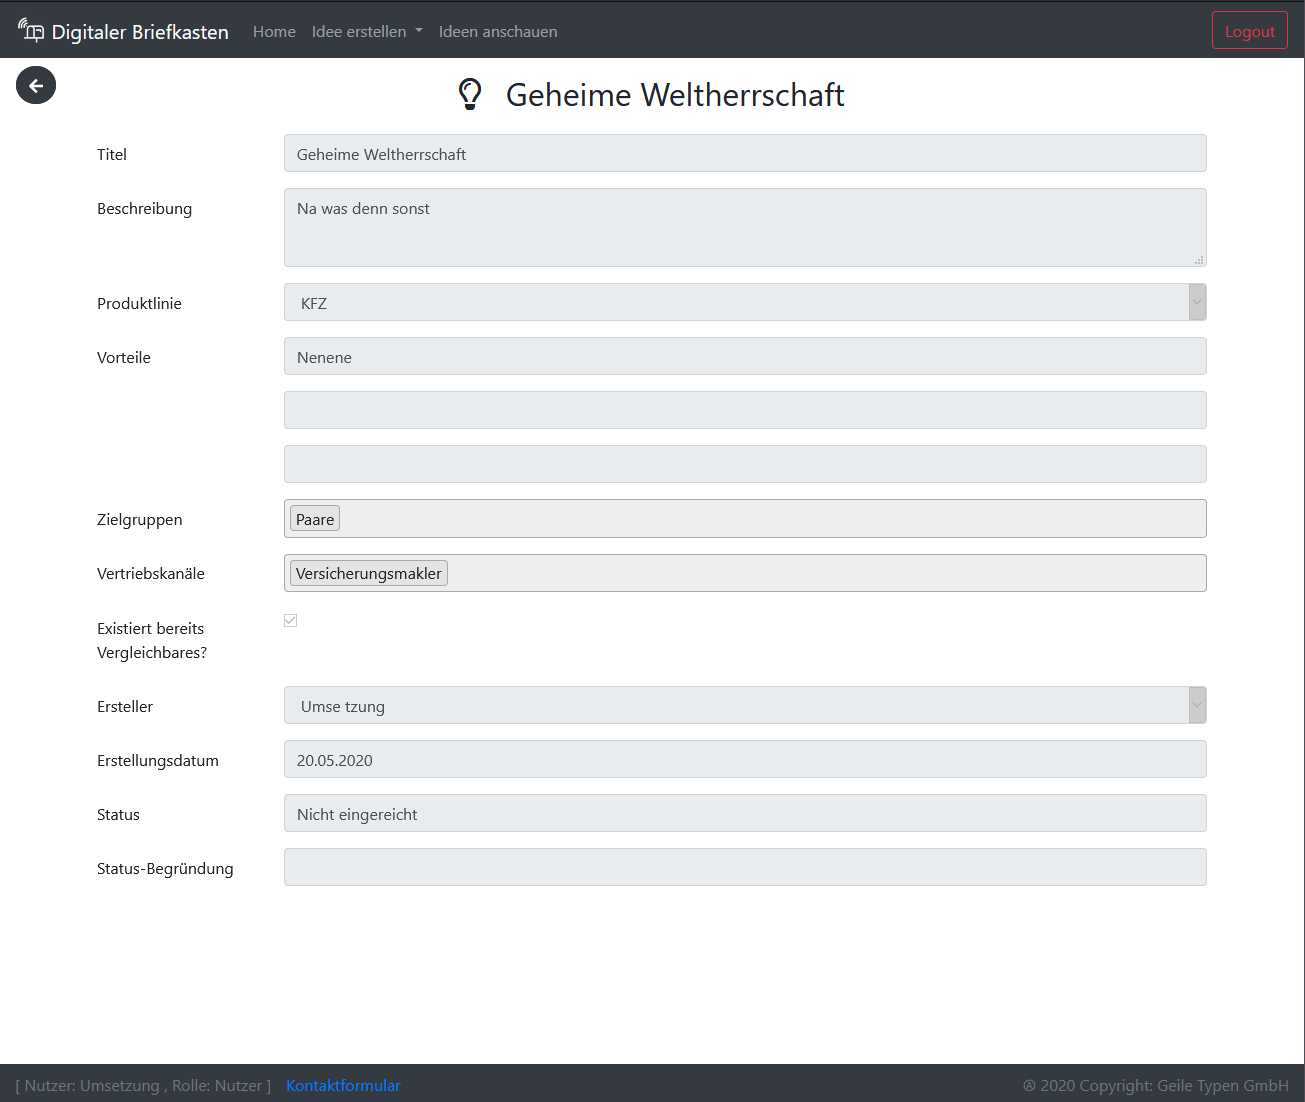
\includegraphics[width=1\textwidth]{img/idee-umsetzung.png}\\
\source{Eigene Darstellung} 
\end{minipage}
\end{figure}

\begin{figure}[h]
\centering
\begin{minipage}[t]{1\textwidth} 
\caption{GUI-Umsetzung - Admin Ansicht } 
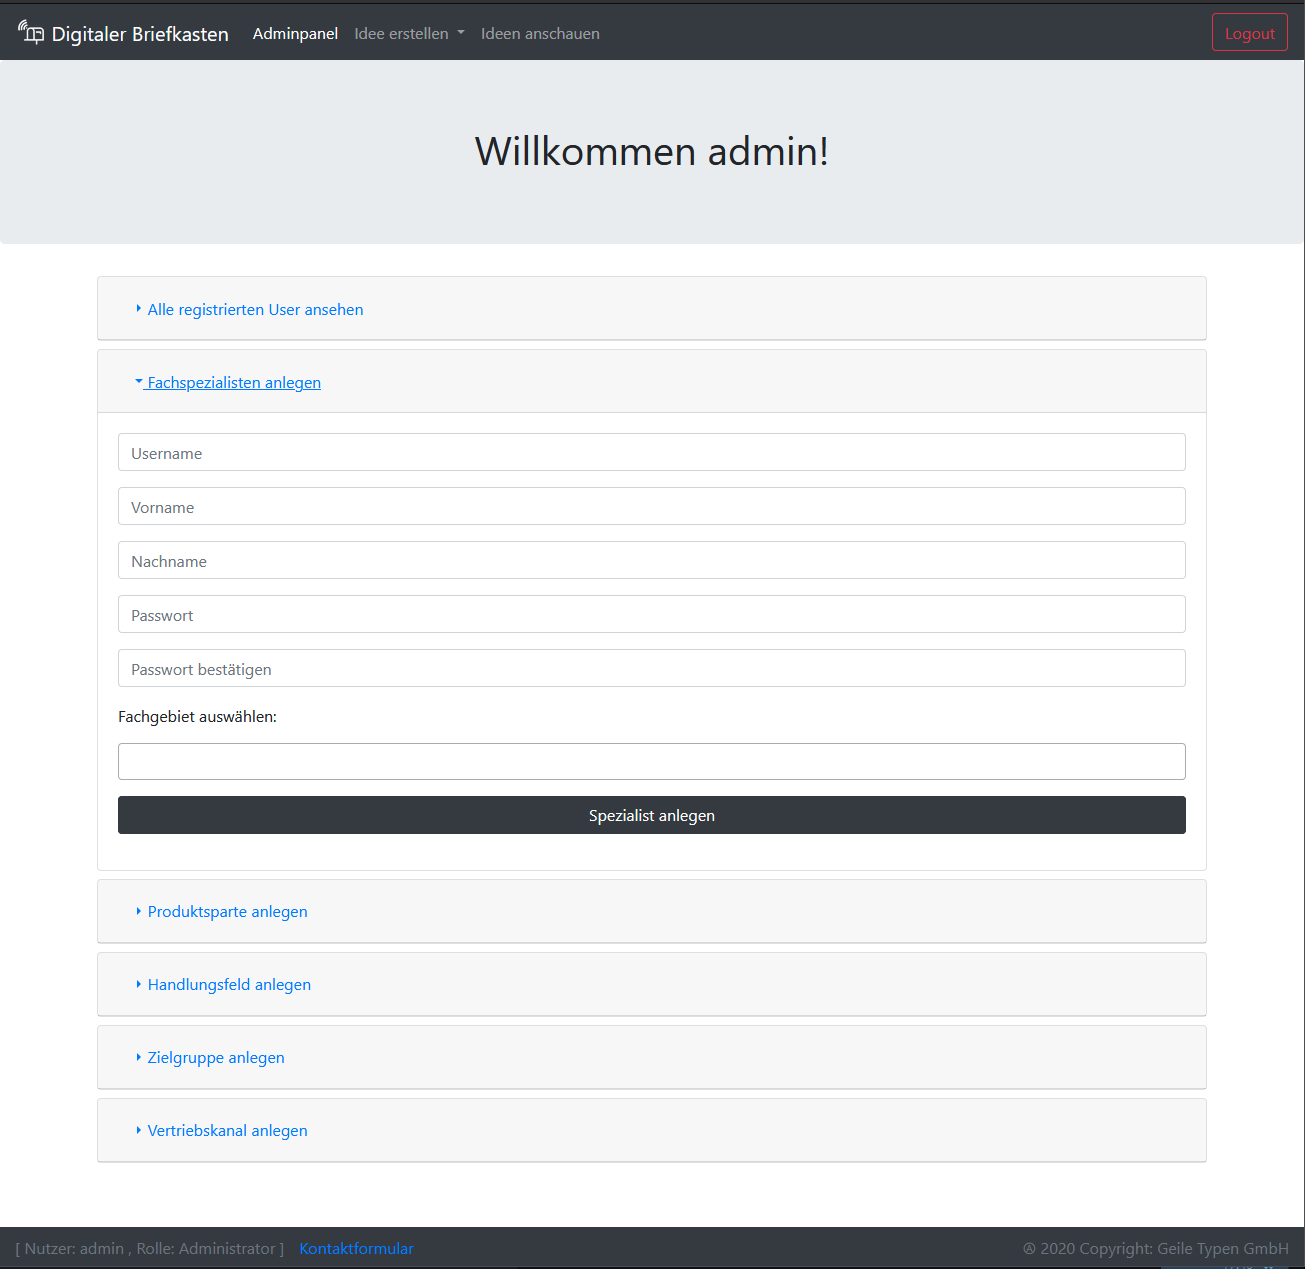
\includegraphics[width=1\textwidth]{img/admin-umsetzung.png}\\
\source{Eigene Darstellung} 
\end{minipage}
\end{figure}

\begin{figure}[h]
    \centering
    \begin{minipage}[t]{1\textwidth}
        \caption{GUI-Umsetzung - Spezialist Ansicht }
        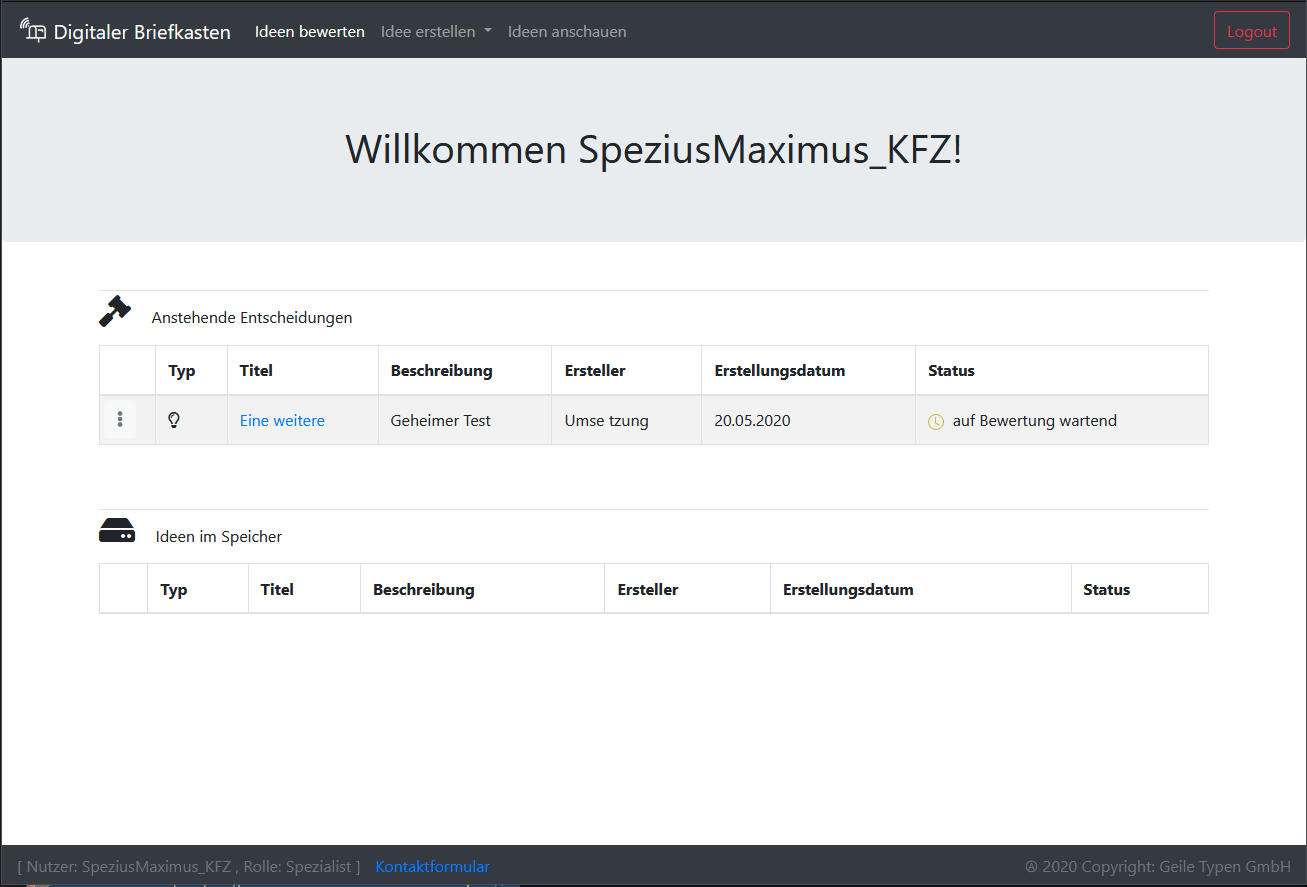
\includegraphics[width=1\textwidth]{img/spezialist-umsetzung.png}\\
        \source{Eigene Darstellung}
    \end{minipage}
\end{figure}

\pagebreak
\clearpage

\anhang{Projektplanung}
\subanhang{Projektstrukturplan}
\label{PSP}
\begin{figure}[h]
    \centering
    \begin{minipage}[t]{1\textwidth}
        \caption{Projektstrukturplan}
        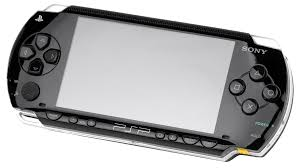
\includegraphics[width=1\textwidth]{img/psp.jpg}\\%TODO Jonathan fix me - Pictures need to be commited...
        \source{Eigene Darstellung}
    \end{minipage}
\end{figure}

\pagebreak
\clearpage
\begin{center}
    \begin{tabularx}{\linewidth}{
        |p{\dimexpr.09\linewidth-2\tabcolsep-1.3333\arrayrulewidth}% column 2
        |p{\dimexpr.71\linewidth-2\tabcolsep-1.3333\arrayrulewidth}% column 1
        |p{\dimexpr.2\linewidth-2\tabcolsep-1.3333\arrayrulewidth}|% column 3
    }
        \hline
        & Anforderung & Umsetzung \\ \hline
        Muss & Noch nicht registrierte Mitarbeiter können sich am System registrieren & Umgesetzt \\ \hline
        Muss & Registrierte Mitarbeiter können sich am System anmelden & Umgesetzt \\ \hline
        Muss & Registrierte Mitarbeiter können neue Ideen erfassen & Umgesetzt \\ \hline
        Muss & Registrierte Mitarbeiter können sich eine Liste ihrer eingereichten Ideen anzeigen lassen & Umgesetzt \\ \hline
        Muss & Registrierte Mitarbeiter können ihre Ideen solange bearbeiten oder auch löschen solange dieses noch nicht zur Bewertung an einen Fachspezialisten übergeben wurden. & Umgesetzt \\ \hline
        Muss & Nicht registrierte Mitarbeiter können vorhandene Ideen lesen, sich eine Übersicht der Ideen anzeigen lassen und die Übersicht filtern & Umgesetzt \\ \hline
        Muss & Diese Funktionen stehen auch registrierten Mitarbeitern zur Verfügung & Umgesetzt \\ \hline
        Muss & Neue Ideen werden Fachspezialisten zur Bewertung zugeordnet & Umgesetzt \\ \hline
        Muss & Die Zuordnung erfolgt automatisch sobald die Idee vom registrierten Mitarbeiter zur Bewertung eingereicht wurde & Umgesetzt \\ \hline
        Muss & Fachspezialisten können eine Idee entweder annehmen, ablehnen oder für einen späteren Zeitpunkt in einen sog. Ideenspeicher überführen / sie aus dem Ideenspeicher zurückholen & Umgesetzt \\ \hline
        Muss & Fachspezialisten begründen ihre Entscheidung transparent und für alle sichtbar in der Anwendung & Umgesetzt \\ \hline
        Muss & Fachspezialisten können ihnen zugewiesene Ideen in einer Liste sehen und diese Liste filtern & Umgesetzt \\ \hline
    \end{tabularx}
\end{center}